\chapter{Genômica e sequenciamento}\label{ch:b3:genomics}

O primeiro genoma completo de um organismo de vida livre, os
\qty{1.8}{Mb} de uma bactéria, foi publicado em 1995 depois de um ano
de trabalho de uma equipe de quarenta pessoas. O genoma humano, com
\num{3.2} bilhões de pares de bases, custou treze anos e cerca de três
bilhões de dólares a um consórcio internacional e foi declarado
concluído em 2003. Hoje uma máquina de bancada lê um genoma humano
numa noite por algumas centenas de dólares, um hospital sequencia o
tumor de um paciente para escolher um fármaco, e um museu extrai e lê
o genoma de um osso de quarenta mil anos. A tecnologia que tornou isso
possível, a matemática que converte milhões de \omterm{def:b3:genomics:ngs}{leituras} curtas num
genoma e o que os genomas prontos ensinaram sobre o tamanho, o
conteúdo e a história de nosso DNA são o assunto deste capítulo. O
capítulo seguinte retoma os algoritmos que comparam as sequências
depois de obtidas.

\section{Ler o DNA}

\begin{definition}[Sequenciamento por terminação de cadeia]\label{def:b3:genomics:sanger}
\index{sequenciamento de Sanger}\index{didesoxinucleotídeo}\index{terminação de cadeia}
O \emph{sequenciamento de Sanger} copia um molde de fita simples a
partir de um iniciador com DNA-polimerase, na presença dos quatro
nucleotídeos normais e de uma pequena proporção de
\emph{didesoxinucleotídeos}, que não têm a hidroxila 3$'$ e por isso
terminam a cadeia onde quer que sejam incorporados. Cada
didesoxinucleotídeo carrega um corante fluorescente diferente. O
produto é uma mistura de fragmentos, um para cada posição do molde,
cada um terminando numa base de identidade conhecida; separados por
tamanho num capilar de gel, eles passam por um detector em ordem de
comprimento, e a sequência de cores é a sequência do molde. Uma
corrida lê \qtyrange{700}{900}{bp} com taxa de erro abaixo de
$10^{-3}$; continua sendo o método para verificar uma construção ou um
gene isolado.
\end{definition}

\begin{proof}[Evidência]
Sanger, Nicklen e Coulson publicaram o método em 1977 e o usaram
naquele mesmo ano para ler os \qty{5386}{bp} do fago $\phi$X174 --- o
primeiro genoma de DNA completo --- e, em 1981, os \qty{16569}{bp} da
mitocôndria humana. Fleischmann e colaboradores (1995) leram os
\qty{1.83}{Mb} de \emph{Haemophilus influenzae} quebrando o genoma
inteiro em fragmentos aleatórios, sequenciando \num{24000} deles e
montando as \omterm{def:b3:genomics:ngs}{leituras} por computador --- a estratégia de
\emph{sequenciamento aleatório do genoma inteiro} que todos os projetos
posteriores ampliaram.
\end{proof}

\begin{omfigure}
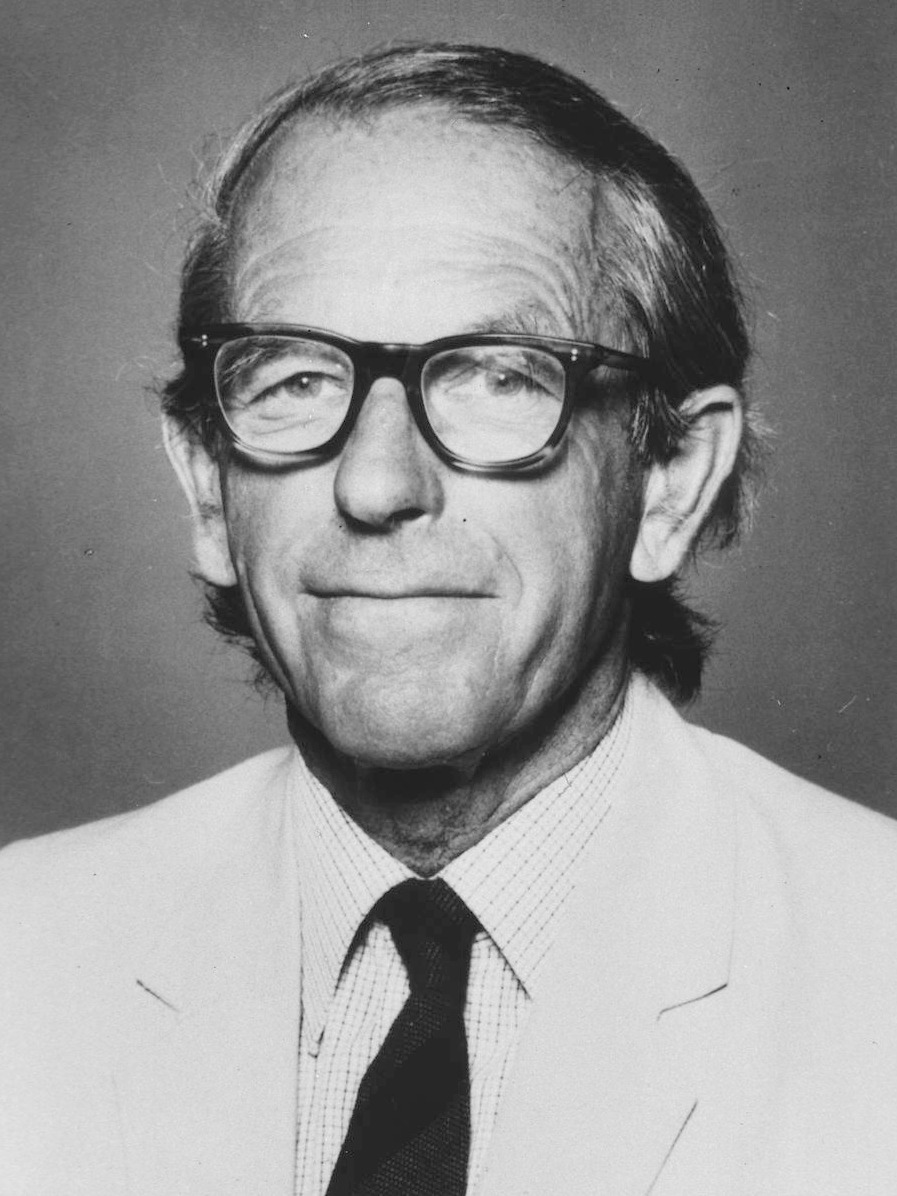
\includegraphics[width=0.30\linewidth]{images/book5/sanger.jpg}\hspace{0.04\linewidth}
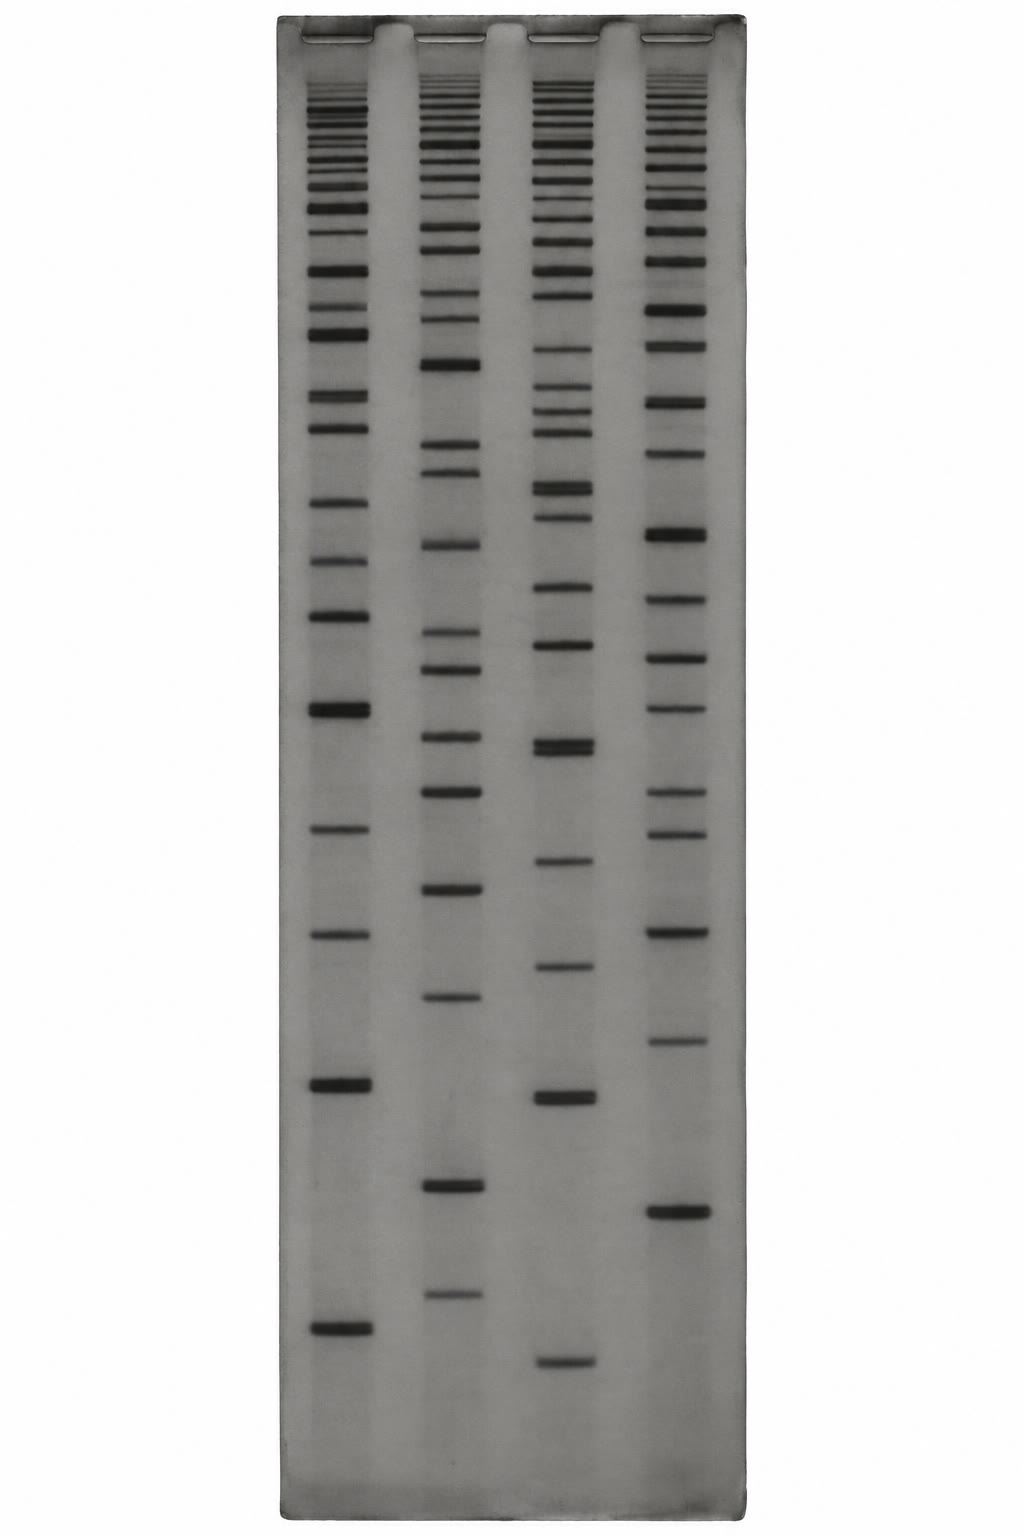
\includegraphics[width=0.30\linewidth]{images/book5/ai/b5-04-sanger-gel.jpg}

{\small À esquerda: Frederick Sanger, que idealizou os primeiros
métodos práticos de \omterm{def:b3:genomics:ngs}{leitura} de proteínas e de DNA e recebeu um prêmio
Nobel por cada um. À direita: uma autorradiografia de um gel de
sequenciamento da era pré-capilar, uma raia por base, com a sequência
lida de baixo para cima na escada de bandas.}
\end{omfigure}

\begin{omfigure}
\begin{tikzpicture}[every node/.style={font=\scriptsize}, >=stealth]
  % template and primer
  \draw[very thick, omDef] (0,3.0) -- (6,3.0); \node[left] at (-0.1,3.0) {molde 3$'$};
  \node[right] at (6.05,3.0) {5$'$};
  \foreach \x/\b in {0.6/T,1.2/G,1.8/A,2.4/C,3.0/T,3.6/T,4.2/G,4.8/C} \node[above, omDef] at (\x,3.05) {\b};
  \draw[very thick, omProp] (0,2.6) -- (0.3,2.6); \node[left] at (-0.1,2.6) {iniciador};
  % terminated products
  \foreach \i/\len/\col/\b in {1/0.6/omDef/A, 2/1.2/omMeth/C, 3/1.8/omThm/T, 4/2.4/omExo/G, 5/3.0/omDef/A, 6/3.6/omDef/A, 7/4.2/omMeth/C, 8/4.8/omExo/G} {
    \draw[very thick, omProp] (0,2.6-0.32*\i) -- (\len-0.15,2.6-0.32*\i);
    \fill[\col] (\len-0.05,2.6-0.32*\i) circle (0.1);
    \node[right, \col] at (\len+0.05,2.6-0.32*\i) {dd\b};
  }
  \node[below, align=center] at (2.4,-0.25) {um produto para cada posição, cada um terminando\\numa base didesoxi fluorescente};
  % capillary readout
  \draw[->, thick] (6.5,1.3) -- (7.4,1.3) node[midway, above] {tamanho};
  \draw[thick] (7.6,0.0) rectangle (11.6,2.6);
  \foreach \i/\col in {1/omDef, 2/omMeth, 3/omThm, 4/omExo, 5/omDef, 6/omDef, 7/omMeth, 8/omExo} {
    \draw[very thick, \col] (7.6+0.45*\i,0.1) .. controls (7.6+0.45*\i-0.15,0.1) and (7.6+0.45*\i-0.1,1.6) .. (7.6+0.45*\i,1.6) .. controls (7.6+0.45*\i+0.1,1.6) and (7.6+0.45*\i+0.15,0.1) .. (7.6+0.45*\i+0.3,0.1);
  }
  \foreach \i/\b in {1/A, 2/C, 3/T, 4/G, 5/A, 6/A, 7/C, 8/G} \node[above] at (7.6+0.45*\i,1.7) {\b};
  \node[below] at (9.6,-0.05) {do mais curto $\to$ ao mais longo: a sequência, lida em cores};
\end{tikzpicture}

{\small Sequenciamento por \omterm{def:b3:genomics:sanger}{terminação de cadeia}. Uma base didesoxi
encerra a cópia em cada posição onde é incorporada; os fragmentos, um
por comprimento, são separados por tamanho e a cor de cada base
terminal é lida em ordem.}
\end{omfigure}

\begin{definition}[Sequenciamento massivamente paralelo]\label{def:b3:genomics:ngs}
\index{sequenciamento por síntese}\index{leitura}\index{sequenciamento de leituras longas}\index{nanoporo}
Os instrumentos de segunda geração leem de milhões a bilhões de
fragmentos ao mesmo tempo. No \emph{sequenciamento por síntese} os
fragmentos, com adaptadores ligados às suas extremidades, são fixados
numa célula de fluxo de vidro e amplificados no lugar em aglomerados
de moléculas idênticas; os aglomerados são então estendidos uma base
por ciclo com nucleotídeos fluorescentes reversivelmente bloqueados,
fotografados, desbloqueados e estendidos de novo, de modo que cada
ciclo acrescenta uma base à \emph{leitura} de cada aglomerado. As
leituras têm \qtyrange{100}{300}{bp}, em geral vindas das duas pontas
de um fragmento (\emph{extremidades pareadas}), com taxa de erro de
cerca de $10^{-3}$ por base, e uma corrida dá até $10^{12}$ bases. Os
instrumentos de terceira geração, de \emph{leituras longas}, leem
moléculas isoladas sem amplificação: observando uma polimerase
incorporar nucleotídeos fluorescentes em tempo real, ou passando o DNA
por um \emph{nanoporo} proteico e registrando a corrente iônica, que
cada sequência de bases modula a seu modo. Leituras de
\qtyrange{10}{100}{kb} e mais atravessam as repetições que as leituras
curtas não vencem, a uma taxa bruta de erro maior que o consenso
reduz.
\end{definition}

\begin{omfigure}
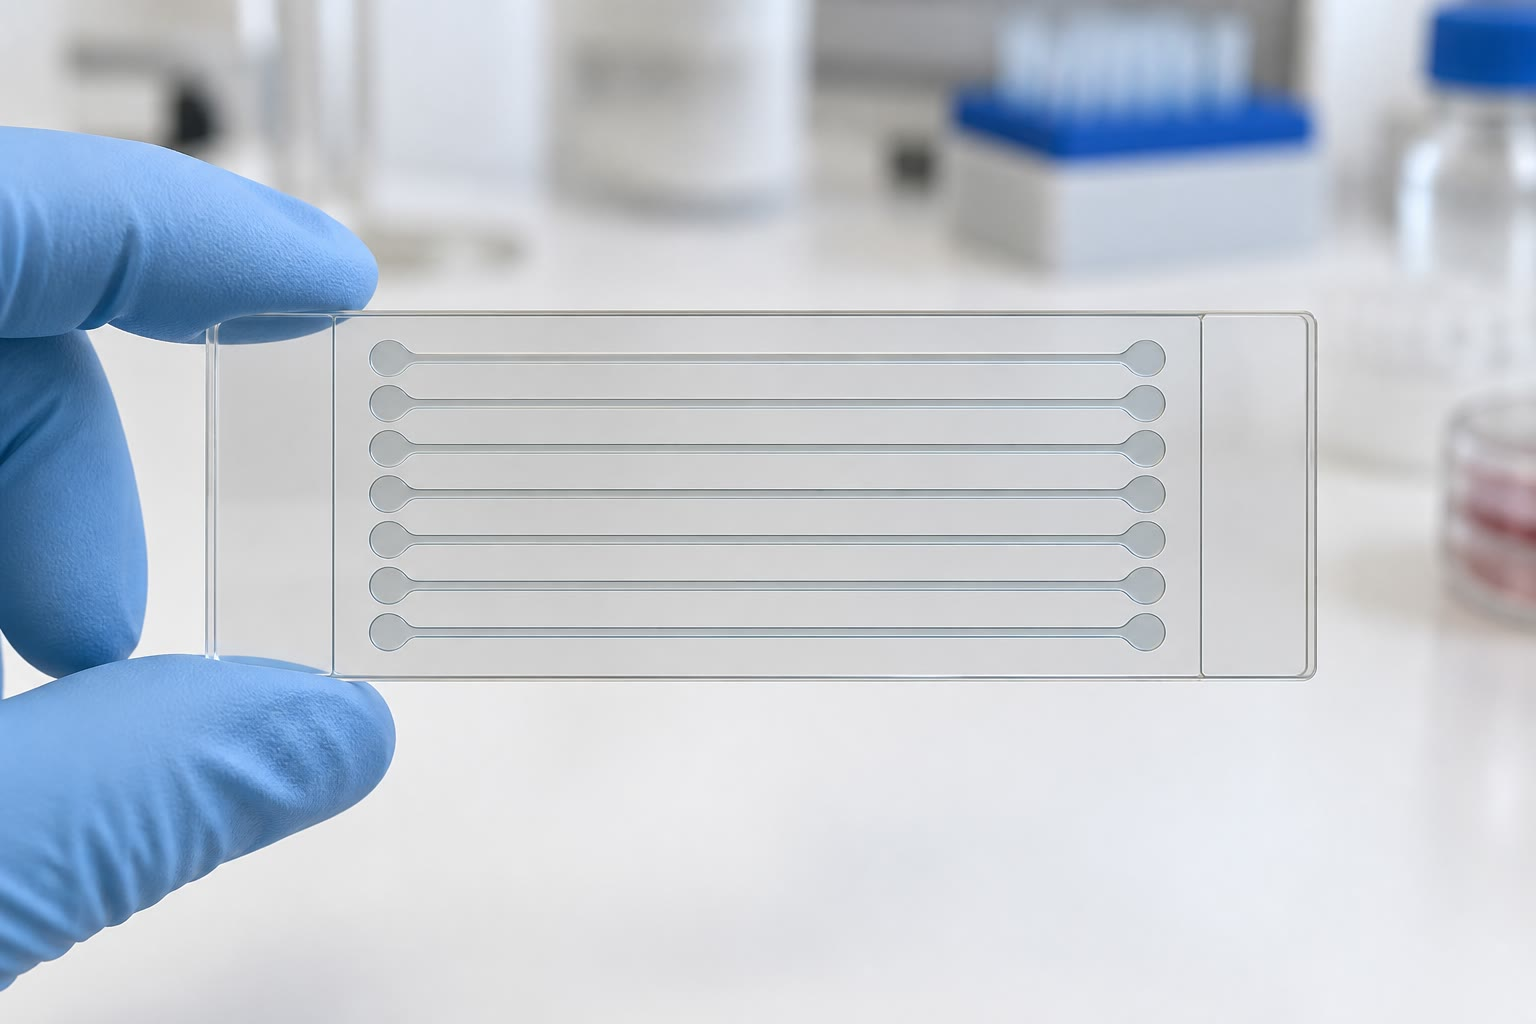
\includegraphics[width=0.46\linewidth]{images/book5/ai/b5-04-flowcell.jpg}\hspace{0.04\linewidth}

\includegraphics[width=0.46\linewidth]{images/book5/ai/b5-04-nanopore.jpg}

{\small À esquerda: uma célula de fluxo, a lâmina de vidro sobre a qual
bilhões de aglomerados de DNA são crescidos e lidos uma base por
ciclo. À direita: um sequenciador de \omterm{def:b3:genomics:ngs}{nanoporo} do tamanho de um bolso,
lendo moléculas isoladas como variações de uma corrente iônica.}
\end{omfigure}

\begin{theorem}[Cobertura e lacunas num projeto de sequenciamento aleatório]\label{thm:b3:genomics:lander-waterman}
\index{cobertura}\index{Lander--Waterman}\index{contig}
Sejam $N$ \omterm{def:b3:genomics:ngs}{leituras} de comprimento $L$ tomadas em posições aleatórias ao
longo de um genoma de comprimento $G$, e seja $c = NL/G$ a
\emph{cobertura}, o número médio de \omterm{def:b3:genomics:ngs}{leituras} que cobrem uma base.
Então uma dada base é coberta por um número de \omterm{def:b3:genomics:ngs}{leituras} que é Poisson
de média $c$: a fração do genoma que fica sem sequenciar é
\[
P(\text{descoberto}) = e^{-c},
\]
e, se duas \omterm{def:b3:genomics:ngs}{leituras} só são reconhecidas como sobrepostas quando
compartilham ao menos $T$ bases, de modo que $\theta = T/L$, o número
esperado de \emph{contigs} (ilhas de \omterm{def:b3:genomics:ngs}{leituras} sobrepostas) é
\[
\text{contigs} = N\,e^{-c(1-\theta)},
\]
e seu comprimento médio é $L\,\bigl(e^{c(1-\theta)} - 1\bigr)/c + L\theta$,
aproximadamente.
\end{theorem}
\begin{proof}
Os pontos de início das \omterm{def:b3:genomics:ngs}{leituras} caem ao acaso com densidade $N/G$ por
base. Uma base é coberta pelas \omterm{def:b3:genomics:ngs}{leituras} que começam nas $L$ bases
anteriores a ela; o número de inícios numa janela de comprimento $L$ é
Poisson de média $LN/G
= c$, e a probabilidade de nenhum é $e^{-c}$.
Uma \omterm{def:b3:genomics:ngs}{leitura} é a mais à direita de seu contig se nenhuma outra \omterm{def:b3:genomics:ngs}{leitura}
começa nas $L - T = L(1-\theta)$ bases depois de seu próprio início
(uma \omterm{def:b3:genomics:ngs}{leitura} que começasse mais tarde a sobreporia em menos de $T$ e
não seria unida); essa probabilidade é $e^{-c(1-\theta)}$ e, como cada
contig tem exatamente uma \omterm{def:b3:genomics:ngs}{leitura} mais à direita, o número esperado de
contigs é $N e^{-c(1-\theta)}$. O comprimento médio do contig segue de
$G$ dividido pelo número de contigs, corrigido pela fração não coberta.
\end{proof}

\begin{example}[Quanto basta]\label{ex:b3:genomics:coverage}
Com $c = 5$ a fração não sequenciada é $e^{-5} = 0.7\,\%$ --- para um
genoma de \qty{3.2}{Gb}, vinte milhões de bases em algumas dezenas de
milhares de lacunas. Com $c = 10$ ela é $4.5\times 10^{-5}$,
\qty{150}{kb} no total. Os genomas humanos são sequenciados de rotina
a $c = 30$, não por causa das lacunas de cobertura
($e^{-30} \approx 10^{-13}$), mas porque cada base precisa ser lida
várias vezes em cada um dos dois cromossomos para que uma variante
heterozigota seja chamada com confiança contra uma taxa de erro de
$10^{-3}$ por \omterm{def:b3:genomics:ngs}{leitura}. Os genomas bacterianos são sequenciados a
$c = 50$--$100$ pela mesma razão e porque é barato. A fórmula também
mostra o que a cobertura não resolve: uma repetição mais longa que uma
\omterm{def:b3:genomics:ngs}{leitura} é um lugar onde o grafo de sobreposições se ramifica, e
nenhuma quantidade de \omterm{def:b3:genomics:ngs}{leituras} curtas a resolve. É para isso que
servem as \omterm{def:b3:genomics:ngs}{leituras} longas.
\end{example}

\begin{omfigure}
\begin{tikzpicture}
\begin{axis}[
  width=0.7\linewidth, height=5.6cm,
  axis x line=bottom, axis y line=left,
  xmin=0, xmax=12, ymin=0.000001, ymax=1, ymode=log,
  xlabel={cobertura $c$}, ylabel={fração},
  xlabel style={font=\small, at={(axis description cs:0.5,-0.12)}, anchor=north},
  ylabel style={font=\small},
  tick label style={font=\small}, xtick={0,2,4,6,8,10,12},
  clip=false,
]
\addplot[very thick, omDef, domain=0:12, samples=40] {exp(-x)};
\addplot[very thick, omThm, domain=0.3:12, samples=40] {exp(-x*0.8)*x/12};
\node[font=\scriptsize, omDef, anchor=north west] at (axis cs:0.3,0.002) {fração não coberta $e^{-c}$};
\node[font=\scriptsize, omThm, anchor=south west] at (axis cs:5.5,0.03) {contigs por leitura $\times\, c/12$, $\theta = 0.2$};
\end{axis}
\end{tikzpicture}

{\small As duas quantidades de Lander--Waterman contra a cobertura: a
fração do genoma que nunca é lida cai como $e^{-c}$, e o número de
contigs (aqui escalonado por \omterm{def:b3:genomics:ngs}{leitura}) tem um pico em cobertura baixa e
depois cai à medida que as ilhas se fundem.}
\end{omfigure}

\section{Das leituras a um genoma}

\begin{definition}[Montagem e anotação]\label{def:b3:genomics:assembly}
\index{montagem}\index{scaffold}\index{N50}\index{anotação}\index{genoma de referência}
A \emph{montagem} reconstrói um genoma a partir de suas \omterm{def:b3:genomics:ngs}{leituras} por
sobreposição: num \emph{grafo de sobreposições} cada \omterm{def:b3:genomics:ngs}{leitura} é um nó
unido às \omterm{def:b3:genomics:ngs}{leituras} que a sobrepõem; num \emph{grafo de de Bruijn},
usado para bilhões de \omterm{def:b3:genomics:ngs}{leituras} curtas, cada $k$-mero (subsequência de
comprimento $k$) é um nó e o genoma é um caminho por eles. Os dois são
rompidos por repetições mais longas que a \omterm{def:b3:genomics:ngs}{leitura}, que dão caminhos
ramificados. Os contigs são ordenados e orientados em \emph{scaffolds}
por \omterm{def:b3:genomics:ngs}{leituras} de extremidades pareadas e por informação de longo
alcance (\omterm{def:b3:genomics:ngs}{leituras} longas, mapas ópticos, mapas de contato
cromossômico), e os scaffolds são colocados nos cromossomos. A
qualidade de uma montagem é resumida pelo \emph{N50}: o comprimento de
contig tal que metade das bases montadas está em contigs pelo menos
tão longos. A \emph{anotação} então localiza os genes: nas bactérias,
fases de \omterm{def:b3:genomics:ngs}{leitura} abertas mais longas do que o acaso daria; nos
eucariontes, combinando sinais de sequência (sítios de splicing,
promotores, viés de códons), homologia com proteínas conhecidas e
transcritos sequenciados a partir do RNA. O resultado, para uma
espécie, é um \emph{genoma de referência} ao qual toda \omterm{def:b3:genomics:ngs}{leitura}
posterior daquela espécie é alinhada, em vez de montada de novo.
\end{definition}

\begin{method}[De uma amostra às variantes]\label{met:b3:genomics:pipeline}
\index{chamada de variantes}
Para um estudo de ressequenciamento de um indivíduo contra uma
referência: (1) extraia o DNA, fragmente-o em \qtyrange{300}{500}{bp}
e ligue adaptadores (a \emph{biblioteca}); (2) sequencie até a
cobertura necessária (30$\times$ para um genoma humano, 100$\times$
para um exoma, que captura os \qty{1.5}{\%} do genoma que codificam
proteína); (3) alinhe cada \omterm{def:b3:genomics:ngs}{leitura} à referência, tolerando
discordâncias; (4) em cada posição conte as bases nas \omterm{def:b3:genomics:ngs}{leituras}: uma
posição em que cerca de metade das \omterm{def:b3:genomics:ngs}{leituras} discorda da referência é
uma \emph{variante} heterozigota, aquela em que quase todas discordam é
homozigota, e aquela em que poucas discordam é erro; (5) filtre por
profundidade, qualidade de base e equilíbrio entre as fitas; (6) anote
cada variante com seu efeito sobre qualquer gene (sinônima, de sentido
trocado, sem sentido, de splicing, de mudança de fase) e com sua
frequência em bancos populacionais; (7) para um diagnóstico, guarde as
variantes raras previstas como danosas em genes compatíveis com o
fenótipo, e confirme por \omterm{def:b3:genomics:sanger}{sequenciamento de Sanger}.
\end{method}

\section{Como são os genomas}

\begin{proposition}[Tamanho do genoma e número de genes]\label{prop:b3:genomics:sizes}
\index{paradoxo do valor C}\index{tamanho do genoma}
Os tamanhos de genoma abrangem um fator de $10^{5}$ entre os
eucariontes --- \qty{12}{Mb} na levedura, \qty{100}{Mb} no verme,
\qty{140}{Mb} na mosca, \qty{3.2}{Gb} num humano, \qty{16}{Gb} numa
cebola, \qty{130}{Gb} num peixe pulmonado, \qty{150}{Gb} no lírio
\emph{Paris japonica} ---, ao passo que os números de genes mal
abrangem um fator de $10$: \num{6000} na levedura, \num{20000} no
verme, \num{14000} na mosca, cerca de \num{20000} genes codificadores
de proteína num humano, \num{40000} no arroz. Este é o \emph{paradoxo
do valor C}: o \omterm{prop:b3:genomics:sizes}{tamanho do genoma} não mede complexidade, e o número de
genes tampouco. O que varia é o conteúdo não codificante --- íntrons,
elementos transponíveis, repetições satélites --- e o número de
proteínas que um genoma pode produzir é multiplicado muito além de sua
contagem de genes pelo splicing alternativo
(\cref{ch:b3:rna-regulation}) e pela regulação, que é onde a
complexidade de um organismo está escrita, na maior parte. Os genomas
bacterianos, em contraste, são compactos, e seu tamanho de fato
acompanha o número de genes: cerca de um gene por quilobase,
\qty{88}{\%} codificante em \emph{E.~coli}.
\end{proposition}

\begin{example}[O genoma humano por conteúdo]\label{ex:b3:genomics:content}
Dos \qty{3.2}{Gb}: éxons codificadores de proteína, \qty{1.5}{\%};
íntrons e regiões não traduzidas dos genes, cerca de \qty{35}{\%};
elementos transponíveis e seus fósseis, cerca de \qty{45}{\%} ---
retrotranspósons LINE-1 \qty{17}{\%}, elementos Alu \qty{10}{\%} (mais
de um milhão de cópias de uma sequência de \qty{300}{bp}), retrovírus
endógenos \qty{8}{\%}; duplicações segmentares \qty{5}{\%}; repetições
simples e satélites, entre elas os centrômeros, cerca de \qty{5}{\%}; o
resto é sequência não codificante única, onde vivem os elementos
regulatórios. Uns \numrange{100}{200} genes ainda codificam uma
maquinaria LINE-1 ativa, e inserções novas ocorrem cerca de uma vez a
cada vinte nascimentos. Cerca de \qty{8}{\%} do genoma está sob
seleção purificadora detectável --- bem mais que os éxons --- e a maior
parte disso é regulatória.
\end{example}

\begin{omfigure}
\begin{tikzpicture}[every node/.style={font=\scriptsize}]
  \def\w{12}
  % stacked bar: fractions
  \fill[omThm] (0,0) rectangle (0.18,0.7);
  \fill[omDef!60] (0.18,0) rectangle (4.38,0.7);
  \fill[omProp!70] (4.38,0) rectangle (6.42,0.7);
  \fill[omProp!45] (6.42,0) rectangle (7.62,0.7);
  \fill[omProp!25] (7.62,0) rectangle (9.78,0.7);
  \fill[omMeth!50] (9.78,0) rectangle (10.38,0.7);
  \fill[gray!45] (10.38,0) rectangle (10.98,0.7);
  \fill[gray!15] (10.98,0) rectangle (12,0.7);
  \draw[thick] (0,0) rectangle (12,0.7);
  % labels above/below with leaders
  \draw (0.09,0.7) -- (0.09,1.1); \node[above, align=center] at (0.5,1.1) {éxons\\\qty{1.5}{\%}};
  \node[above] at (2.3,0.75) {íntrons e UTRs dos genes: \qty{35}{\%}};
  \node[below, align=center] at (5.4,-0.05) {LINE-1\\\qty{17}{\%}};
  \node[below, align=center] at (7.0,-0.05) {Alu\\\qty{10}{\%}};
  \node[below, align=center] at (8.7,-0.05) {outros transpósons,\\retrovírus \qty{18}{\%}};
  \node[above, align=center] at (10.1,0.75) {duplicações\\segmentares \qty{5}{\%}};
  \node[below, align=center] at (10.7,-0.05) {satélites\\\qty{5}{\%}};
  \draw[gray] (11.5,0.72) -- (12.0,1.05); \node[above, align=center] at (12.3,1.05) {outra sequência\\única não codificante};
  \draw[decorate, decoration={brace, amplitude=4pt, mirror}] (4.38,-1.0) -- (9.78,-1.0) node[midway, below=4pt] {derivado de elementos transponíveis: \qty{45}{\%}};
\end{tikzpicture}

{\small O genoma humano por conteúdo, em escala. Os éxons codificadores
de proteína (vermelho) são uma lasca; quase metade do genoma descende
de elementos transponíveis.}
\end{omfigure}

\begin{definition}[Genômica comparativa]\label{def:b3:genomics:comparative}
\index{ortólogo}\index{parálogo}\index{sintenia}\index{elemento não codificante conservado}\index{duplicação do genoma inteiro}
Genes de duas espécies descendentes de um mesmo gene do ancestral
comum são \emph{ortólogos}; genes de uma mesma espécie descendentes de
uma duplicação são \emph{parálogos}. Blocos de cromossomo em que a
ordem dos genes se conserva entre espécies são \emph{sintênicos}; a
sintenia permite localizar um gene num genoma a partir de sua posição
em outro e revela os rearranjos que separam dois cariótipos (cerca de
\num{1000} entre humano e camundongo). As sequências conservadas entre
espécies distantes que não codificam proteína alguma --- os
\emph{elementos não codificantes conservados}, alguns
ultraconservados base a base ao longo de \qty{200}{bp} entre humano e
peixe --- são em sua maioria intensificadores de genes do
desenvolvimento. As \emph{duplicações do genoma inteiro} marcaram a
história de várias linhagens: duas rodadas na origem dos vertebrados
(os quatro agrupamentos Hox dos mamíferos contra o único dos
invertebrados), uma no ancestral dos salmonídeos, uma na linhagem das
leveduras, várias nas plantas com flor; os genes duplicados são em sua
maioria perdidos ao longo de dezenas de milhões de anos, e os
sobreviventes divergem em função.
\end{definition}

\begin{example}[Humano e chimpanzé]\label{ex:b3:genomics:chimp}
A sequência de cópia única alinhada difere entre humano e chimpanzé em
\qty{1.2}{\%} das bases --- uns \num{35} milhões de substituições --- e
por inserções e deleções que juntas somam mais \qty{3}{\%} de cada
genoma. Dois humanos diferem em cerca de uma base em mil, uns
\numrange{4}{5} milhões de sítios, além de alguns milhares de
variantes estruturais; dois chimpanzés, cuja população foi maior por
mais tempo, diferem em bem mais. Uma criança carrega cerca de
\num{70} mutações novas ausentes nos dois pais, quatro quintos delas
vindas do pai, e o número sobe cerca de duas por ano de idade paterna
--- a aritmética do \cref{ch:b3:dna-repair} aplicada às muitas divisões
da espermatogênese.
\end{example}

\section{Genomas e características}

\begin{definition}[Associação genômica ampla]\label{def:b3:genomics:gwas}
\index{estudo de associação genômica ampla}\index{polimorfismo de nucleotídeo único}\index{escore poligênico}
Um \emph{polimorfismo de nucleotídeo único} (SNP) é uma posição em que
duas bases ocorrem, cada uma em ao menos \qty{1}{\%} de uma população;
cerca de dez milhões são comuns nos humanos. Um \emph{estudo de
associação genômica ampla} (GWAS) genotipa centenas de milhares de
SNPs em milhares de pessoas com uma doença e em milhares sem ela, e
pergunta, em cada SNP, se um alelo é mais frequente nos casos. Como se
fazem um milhão de testes, um resultado só conta abaixo de um limiar
de significância de cerca de $5\times 10^{-8}$ ($0.05$ dividido pelo
milhão de testes efetivamente independentes). Os SNPs associados
marcam uma região, e não uma variante causal, já que alelos vizinhos
viajam juntos (desequilíbrio de ligação) ao longo de dezenas de
quilobases. Para a maioria das doenças comuns, cada alelo associado
desloca o risco em poucos por cento e a maior parte deles está em
sequência regulatória; seu efeito combinado, somado ao longo de
milhares de SNPs como um \emph{escore poligênico}, explica uma fração
da herdabilidade e prevê o risco mais ou menos tão bem quanto a
história familiar.
\end{definition}

\begin{remark}[O que a genômica entregou e o que não entregou]\label{rem:b3:genomics:delivered}
O sequenciamento foi decisivo onde um único gene tem grande efeito:
vários milhares de doenças mendelianas já têm seu gene, e sequenciar o
exoma de uma criança com um distúrbio sem diagnóstico dá um
diagnóstico em cerca de um terço dos casos. Os genomas de tumores
revelam quais condutores um tumor carrega e quais fármacos podem
funcionar (\cref{ch:b3:cancer-biology}); os genomas de patógenos
rastreiam surtos linhagem por linhagem (\cref{ch:b3:bacteriology}); os
genomas antigos reescreveram a pré-história humana, mostrando que as
pessoas de fora da África carregam cerca de \qty{2}{\%} de DNA
neandertal. Para as doenças comuns --- diabetes, doença cardíaca,
esquizofrenia --- a genômica entregou milhares de efeitos pequenos e
poucos mecanismos, e a promessa de prever a partir do genoma de uma
pessoa saudável continua modesta. O genoma é uma lista de peças; a
biologia de como as peças interagem não se lê nele.
\end{remark}

\section{Exercícios}

\begin{exercise}[$\star$]\label{exo:b3:genomics:1}
Explique por que um \omterm{def:b3:genomics:sanger}{didesoxinucleotídeo} termina uma cadeia de DNA em
crescimento, e por que uma reação de Sanger precisa conter as formas
normal e didesoxi de cada nucleotídeo.
\end{exercise}

\begin{exercise}[$\star$]\label{exo:b3:genomics:2}
Uma corrida produz $4\times 10^{8}$ \omterm{def:b3:genomics:ngs}{leituras} pareadas de
$2\times \qty{150}{bp}$. Que cobertura isso dá de um genoma humano de
\qty{3.2}{Gb}? E de um genoma bacteriano de \qty{5}{Mb}?
\end{exercise}

\begin{exercise}[$\star$]\label{exo:b3:genomics:3}
Defina contig, \omterm{def:b3:genomics:assembly}{scaffold} e \omterm{def:b3:genomics:assembly}{N50}. Uma \omterm{def:b3:genomics:assembly}{montagem} de \qty{100}{Mb} tem dez
contigs de \qty{8}{Mb} e \num{2000} de \qty{10}{kb}. Qual é seu \omterm{def:b3:genomics:assembly}{N50}?
\end{exercise}

\begin{exercise}[$\star$]\label{exo:b3:genomics:4}
Enuncie o paradoxo do valor C com dois exemplos, e diga o que responde
principalmente pelo DNA em excesso dos genomas grandes.
\end{exercise}

\begin{exercise}[$\star\star$]\label{exo:b3:genomics:5}
Usando o \cref{thm:b3:genomics:lander-waterman}, determine a cobertura
necessária para deixar no máximo uma base em um milhão sem sequenciar,
e o número esperado de contigs de um genoma de \qty{5}{Mb} lido a
$c = 8$ com \omterm{def:b3:genomics:ngs}{leituras} de \qty{150}{bp} e sobreposição mínima de
\qty{30}{bp}.
\end{exercise}

\begin{exercise}[$\star\star$]\label{exo:b3:genomics:6}
Uma variante heterozigota é coberta por $30$ \omterm{def:b3:genomics:ngs}{leituras}. Supondo que
cada \omterm{def:b3:genomics:ngs}{leitura} mostre um dos alelos com probabilidade $1/2$, qual é a
probabilidade de menos de $8$ \omterm{def:b3:genomics:ngs}{leituras} mostrarem o alelo variante (de
modo que ele pudesse ser tomado por erro)? Use uma aproximação normal
com média $15$ e desvio padrão $\sqrt{7.5}$. Por que $30\times$ é o
padrão?
\end{exercise}

\begin{exercise}[$\star\star$]\label{exo:b3:genomics:7}
Um genoma tem uma repetição de \qty{6}{kb} presente em \num{500}
cópias. Explique por que uma \omterm{def:b3:genomics:assembly}{montagem} a partir de \omterm{def:b3:genomics:ngs}{leituras} de
\qty{150}{bp} a colapsa, como fica o grafo resultante e que comprimento
de \omterm{def:b3:genomics:ngs}{leitura} a resolveria.
\end{exercise}

\begin{exercise}[$\star\star$]\label{exo:b3:genomics:8}
Dois humanos diferem em uma base em mil. Quantas diferenças há em seus
exomas (\qty{48}{Mb} de sequência codificadora)? Se dois terços das
diferenças codificadoras são sinônimas ou benignas e o resto altera
uma proteína, quantas variantes que alteram proteína uma pessoa
carrega em relação a outra?
\end{exercise}

\begin{exercise}[$\star\star$]\label{exo:b3:genomics:9}
Um GWAS testa $10^{6}$ SNPs com limiar $p < 5\times 10^{-8}$. Quantos
falsos positivos se esperam se nenhum SNP estiver de fato associado?
Um alelo de SNP eleva o risco de uma doença de frequência \qty{2}{\%}
para \qty{2.3}{\%}. Explique por que um efeito desses é indetectável
num estudo de mil pessoas e inútil para um indivíduo, mas pode ainda
assim apontar para um mecanismo.
\end{exercise}

\begin{exercise}[$\star\star\star$]\label{exo:b3:genomics:10}
Os genomas bacterianos são cerca de \qty{88}{\%} codificantes; o
genoma humano, \qty{1.5}{\%}. Dê três hipóteses --- de genética de
populações, estrutural e regulatória --- para a diferença e, para cada
uma, uma observação genômica que a apoie ou a enfraqueça.
\end{exercise}

\begin{exercise}[$\star\star\star$]\label{exo:b3:genomics:11}
Deduza a contagem de contigs de Lander--Waterman para \omterm{def:b3:genomics:ngs}{leituras} de dois
comprimentos misturados: $N_{1}$ \omterm{def:b3:genomics:ngs}{leituras} curtas de comprimento
$L_{1}$ e $N_{2}$ \omterm{def:b3:genomics:ngs}{leituras} longas de comprimento $L_{2}$, com as
sobreposições contadas com o mesmo mínimo $T$. (Trate cada \omterm{def:b3:genomics:ngs}{leitura}
como a mais à direita de seu contig se nenhuma \omterm{def:b3:genomics:ngs}{leitura} de qualquer dos
tipos começa dentro de seu próprio comprimento menos $T$.) Mostre que
algumas poucas \omterm{def:b3:genomics:ngs}{leituras} longas reduzem a contagem de contigs mais do
que o mesmo número de bases em \omterm{def:b3:genomics:ngs}{leituras} curtas.
\end{exercise}

\begin{exercise}[$\star\star\star$]\label{exo:b3:genomics:12}
Argumenta-se que os quatro agrupamentos Hox dos mamíferos descendem de
um só agrupamento por duas rodadas de \omterm{def:b3:genomics:comparative}{duplicação do genoma inteiro} na
base dos vertebrados. Diga que padrão de \omterm{def:b3:genomics:comparative}{parálogos} pelo genoma, e que
padrão nos genomas das lampreias e dos cordados invertebrados, essa
hipótese prevê, e como se a distinguiria de duas duplicações
independentes só do agrupamento.
\end{exercise}

\section{Problema: dois genomas numa máquina}

\begin{problem}[{Problema de fim de semana --- uma bactéria e um humano
sequenciados na mesma corrida: as leituras repartidas, a cobertura e as
lacunas calculadas, os contigs contados, as variantes heterozigotas
chamadas contra a taxa de erro, o conteúdo do genoma humano pesado e um
estudo de associação dimensionado, terminando na contagem de contigs em
cobertura baixa, na cobertura que torna segura a chamada de uma
variante e no número de mutações novas numa criança}]
\label{pb:b3:genomics:1}
Dados: uma corrida dá $6\times 10^{8}$ \omterm{def:b3:genomics:ngs}{leituras} de \qty{150}{bp}. Um
genoma bacteriano tem \qty{4.6}{Mb}; o genoma humano, \qty{3.2}{Gb}
(haploide). Sobreposição mínima $T = \qty{30}{bp}$. Taxa de erro
$10^{-3}$ por base por \omterm{def:b3:genomics:ngs}{leitura}. Sequência codificadora humana
\qty{48}{Mb}; o genoma é \qty{45}{\%} derivado de transpósons, com
$1.1$ milhão de cópias Alu de \qty{300}{bp}. Dois humanos diferem em um
sítio em \num{1000}. Taxa de mutação $1.2\times 10^{-8}$ por base por
geração.

\medskip
\noindent\textbf{Parte I --- A bactéria.}
\begin{enumerate}
  \item A bactéria recebe \qty{0.2}{\%} da corrida. Quantas \omterm{def:b3:genomics:ngs}{leituras}, e
        que cobertura?
  \item Que fração de seu genoma fica sem sequenciar? Quantas bases são
        essas?
  \item Calcule $\theta$ e o número esperado de contigs.
  \item Um ensaio piloto anterior usou apenas \num{30000} \omterm{def:b3:genomics:ngs}{leituras}.
        Cobertura, fração não coberta e número de contigs?
  \item O genoma contém \num{7} cópias de um óperon de rRNA de
        \qty{5}{kb}. Explique o que acontece com elas na \omterm{def:b3:genomics:assembly}{montagem} e
        quantas pontas de contig só isso produz.
  \item A bactéria tem cerca de um gene por quilobase. Quantos genes e,
        se \qty{88}{\%} do genoma é codificante, qual é o comprimento
        médio de um gene?
\end{enumerate}

\medskip
\noindent\textbf{Parte II --- O humano.}
\begin{enumerate}[resume]
  \item O resto da corrida vai para um genoma humano. Qual a cobertura
        do genoma diploide por cópia haploide (isto é, o total de bases
        dividido por \qty{3.2}{Gb})?
  \item Num sítio heterozigoto cada um dos dois alelos é coberto por
        cerca de metade das \omterm{def:b3:genomics:ngs}{leituras}. Com a cobertura da questão 7,
        qual é o número esperado de \omterm{def:b3:genomics:ngs}{leituras} que mostram cada alelo?
  \item Um erro mostra uma base errada numa \omterm{def:b3:genomics:ngs}{leitura} com probabilidade
        $10^{-3}$. Num sítio homozigoto coberto por $c$ \omterm{def:b3:genomics:ngs}{leituras}, qual
        é o número esperado de \omterm{def:b3:genomics:ngs}{leituras} que mostram uma base errada
        qualquer em particular ($10^{-3}/3$ cada)? Por que uma regra
        ``chame uma variante se ao menos $3$ \omterm{def:b3:genomics:ngs}{leituras} e ao menos
        \qty{20}{\%} das \omterm{def:b3:genomics:ngs}{leituras} a mostrarem'' rejeita os erros nessa
        cobertura?
  \item Quantos sítios heterozigotos um humano carrega (metade das
        diferenças entre dois genomas aleatórios está em cada um,
        grosso modo: tome um sítio em \num{1500})? Quantos em sequência
        codificadora?
  \item As \omterm{def:b3:genomics:ngs}{leituras} são alinhadas a uma referência. Explique por que as
        \omterm{def:b3:genomics:ngs}{leituras} vindas de elementos Alu muitas vezes se alinham à
        cópia errada e que consequência isso tem para a \omterm{met:b3:genomics:pipeline}{chamada de
        variantes} dentro deles.
  \item Uma criança é sequenciada junto com os dois pais. Quantas
        mutações novas você espera? Quantas \omterm{def:b3:genomics:ngs}{leituras} na criança, nessa
        cobertura, precisam mostrar uma variante ausente nos
        \emph{dois} pais para que ela seja aceita, e por que a
        cobertura dos pais é tão importante quanto a da criança?
  \item Um laboratório clínico captura o exoma (\qty{48}{Mb}) e o
        sequencia a $100\times$. Quantas \omterm{def:b3:genomics:ngs}{leituras} isso exige, e por que
        sai mais barato por paciente do que um genoma a $28\times$,
        embora sua cobertura seja maior?
\end{enumerate}

\medskip
\noindent\textbf{Parte III --- O conteúdo de um genoma.}
\begin{enumerate}[resume]
  \item Que fração do genoma humano é Alu, e que fração das \omterm{def:b3:genomics:ngs}{leituras} da
        questão 7 vem de elementos Alu?
  \item A referência tem \qty{3.2}{Gb}, mas uma célula diploide contém
        \qty{6.4}{Gb}; e uma cebola de \qty{16}{Gb} tem cerca de
        \num{60000} genes. Qual é a fração codificante do genoma da
        cebola, se seus genes têm em média \qty{1.5}{kb} de sequência
        codificadora?
  \item Humano e chimpanzé diferem em \qty{1.2}{\%} das bases
        alinhadas. Quantas substituições são essas em \qty{2.9}{Gb} de
        sequência alinhável? Repartidas igualmente entre as duas
        linhagens ao longo de $6.5$ milhões de anos, que taxa de
        mutação por base por ano isso implica, e por geração de $25$
        anos? Compare com a medida direta dada nos dados.
  \item Duas duplicações do genoma dos vertebrados deveriam dar até
        quatro cópias de cada gene ancestral. Os humanos têm cerca de
        \num{20000} genes e o cordado invertebrado \emph{Ciona} cerca
        de \num{16000}. Que fração das duplicatas se perdeu, sob a
        hipótese de que o ancestral tinha \num{16000}?
  \item Explique por que o número de genes é uma medida ruim de
        complexidade do organismo, usando a contagem de splicing
        alternativo do \cref{ch:b3:rna-regulation} como um argumento.
  \item \qty{8}{\%} do genoma está sob seleção purificadora, mas apenas
        \qty{1.5}{\%} codifica proteína. O que provavelmente é o resto,
        e como você testaria um elemento candidato?
\end{enumerate}

\medskip
\noindent\textbf{Parte IV --- Um estudo de associação.}
\begin{enumerate}[resume]
  \item $10^{6}$ SNPs são testados. Enuncie o limiar de Bonferroni para
        um erro por família de $0.05$, e o número esperado de falsos
        positivos a $p < 10^{-5}$.
  \item Uma doença tem prevalência de \qty{1}{\%}. Um alelo de risco de
        frequência $0.3$ eleva as chances em \qty{5}{\%}. Calcule o
        risco da doença para um portador de duas cópias, de uma cópia e
        de nenhuma, tomando o risco do não portador como \qty{0.9}{\%}.
        (Multiplique as chances.)
  \item Duzentos alelos desses são encontrados. Explique o que é um
        \omterm{def:b3:genomics:gwas}{escore poligênico} e por que o escore de uma pessoa no
        \qty{1}{\%} mais alto pode corresponder a um risco várias vezes
        maior, embora cada alelo quase nada faça.
  \item Explique por que um SNP que alcança significância em geral não
        é a variante causal, e que experimento identificaria a causal
        na região.
  \item Um genoma antigo de um osso de \num{40000} anos é sequenciado a
        $c = 0.5$. Que fração dele é lida? Por que isso ainda pode
        responder a perguntas sobre história populacional que um genoma
        moderno sozinho não responde?
  \item Resuma: o número de contigs da \omterm{def:b3:genomics:assembly}{montagem} piloto (questão~4), a
        cobertura por genoma haploide que dá cerca de $15$ \omterm{def:b3:genomics:ngs}{leituras} por
        alelo (questões~7--8) e o número de mutações novas numa criança
        (questão~12).
\end{enumerate}
\end{problem}
